\section{Arduino Sensor Gas}
\subsection{Pengertian Arduino}
Arduino adalah perusahaan perangkat keras dan perangkat lunak komputer open-source, proyek, dan komunitas pengguna yang merancang dan memproduksi mikrokontroler board tunggal dan kit mikrokontroler untuk membangun perangkat digital dan objek interaktif yang dapat merasakan dan mengendalikan objek di dunia fisik.
Arduino juga merupakan platform perangkat keras terbuka yang ditujukan untuk siapa pun dan kalangan apapun yang ingin membuat prototip peralatan elektronik interaktif berdasarkan perangkat keras dan perangkat lunak yang fleksibel dan mudah digunakan. Perangkat dari mikrokontroler deprogram atau dibuat menggunakan bahasa pemrograman arduino yang memiliki kesamaan atau kemiripan dengan bahasa pemrograman C, karena bersifat terbuka dapat mendownload skema hardware arduino dan membangunnya. 
Arduino menggunakan keluarga mikrokontroler ATMega yang dilepaskan Atmel sebagai basis, namun ada individu perusahaan yang membuat klon arduino menggunakan mikrokontroler lainnya dan tetap kompatibel dengan arduino di tingkat perangkat keras. Agar bisa, program dimuatkan melalui bootloader meski ada pilihan untuk bypass bootloader dan menggunakan downloader untuk memprogram mikrokontroler secara langsung melalui port ISP.
Produk proyek didistribusikan sebagai perangkat keras dan perangkat lunak open-source, yang berlisensi di bawah GNU Lesser General Public License atau GNU General Public License GPL, yang mengizinkan pembuatan papan Arduino dan distribusi perangkat lunak oleh siapa saja. Papan Arduino tersedia secara komersil dalam bentuk preassembled, atau sebagai kit do-it-yourself. \cite{kushner2011making}
\subsection{sensor gas}
Sensor yang digunakan kali ini adalah sensor MQ-2, sensor ini digunakan untuk mendeteksi gas LPG, i-butana, propana, alkohol, hidroge, dan asap. Inti dari MQ-2 adalah material yang sensitif terhadap konsentrasi gas yang tersusun dari senyawa SnO2 atau Timah Oksida. Material ini mempunyai karakteristik yang akan merubah konduktivitasnya seiring dengan perubahan konsenterasi gas.
Seri MQ sensor gas menggunakan pemanas kecil di dalamnya dengan sensor elektro-kimia. Mereka sensitif terhadap berbagai gas dan digunakan di dalam ruangan pada suhu kamar.
Mereka dapat dikalibrasi lebih atau kurang lihat bagian tentang Load-resistor dan Burn-in namun diketahui konsentrasi gas atau gas yang diukur diperlukan untuk itu.
Outputnya adalah sinyal analog dan bisa dibaca dengan input analog Arduino.
Sedangkan untuk spesifikasi sensor MQ-2, adalah:
\begin{itemize}
\item suhu 20 derajat Celcius
\item kelembaban udara 65 persen
\end{itemize}
range konsentrasi gas yang bisa diukur:
\begin{itemize}
\item LPG dan propana: 200ppm-5000ppm
\item butana: 300ppm-5000ppm
\item metana: 5000ppm - 20000ppm
\end{itemize}

\subsection{hardware yang digunakan}
Perangkat Keras Sistem pengukuran kami terdiri dari beberapa bagian. Kami menggunakan modul sensor MQ-2 untuk merasakan gas. Komunikasi digital dimungkinkan melalui antarmuka RS232 board. Arduino Uno board terhubung ke modul sensor gas MQ2 dan terhubung melalui USB ke sistem komputer untuk mencatat data real-time dari sensor. Semua bagian praktikum ini termasuk modul sensor dan arduino mudah didapat dengan harga murah. Hal ini penting untuk mendapatkan penerimaan yang luas terhadap sistem pemantauan asap.
	
\subsection{Koneksi Sensor Modul}
Sambungan modul sensor Modul sensor gas MQ2 terhubung ke papan Arduino menggunakan kabel jumper. Pin Analog pada sensor terhubung ke pin analog 0 pada papan arduino, sedangkan pin 5 V dan GND pada modul sensor terhubung ke pin 5V Vcc dan GND masing-masing pada papan arduino. Arduino Uno board kemudian dihubungkan ke sistem komputer dengan menggunakan koneksi USB dan antarmuka RS232.

\subsection{Eksperimen}
Alat dan bahan:
\begin{enumerate}
\item Arduino Uno
\item Sensor Gas MQ
\item Led
\item Kabel Jumper
\item Breadboard
\item Resistor
\item Gas korek api
\end{enumerate}
Kode
\begin{verbatim}
int redLed = 12;
int redLed = 11;
int redLed = 10;
int smokeA0 = A5;
// Your threshold value
int sensorThres = 400;

void setup() {
  pinMode(redLed, OUTPUT);
  pinMode(redLed, OUTPUT);
  pinMode(redLed, OUTPUT);
   pinMode(smokeA0, INPUT);
  Serial.begin(9600);
}

void loop() {
  int analogSensor = analogRead(smokeA0);

  Serial.print("Pin A0: ");
  Serial.println(analogSensor);
  // Checks if it has reached the threshold value
  if (analogSensor > sensorThres)
  {
    digitalWrite(redLed, HIGH);
    digitalWrite(redLed, LOW);
    digitalWrite(redLed, HIGH);
  }
  else
  {
    digitalWrite(redLed, LOW);
    digitalWrite(redLed, HIGH);
    digitalWrite(redLed, LOW);
  }
  delay(100);
}
\end{verbatim}

Keadaan sensor jika mendeteksi gas ada pada gambar \ref{sensor:terditeksi} dua lampu akan menyala, sedangkan jika tidak, dua lampu akan padam seperti pada gambar \ref{sensor:tidakterditeksi}

\begin{figure}[ht]
	\centerline{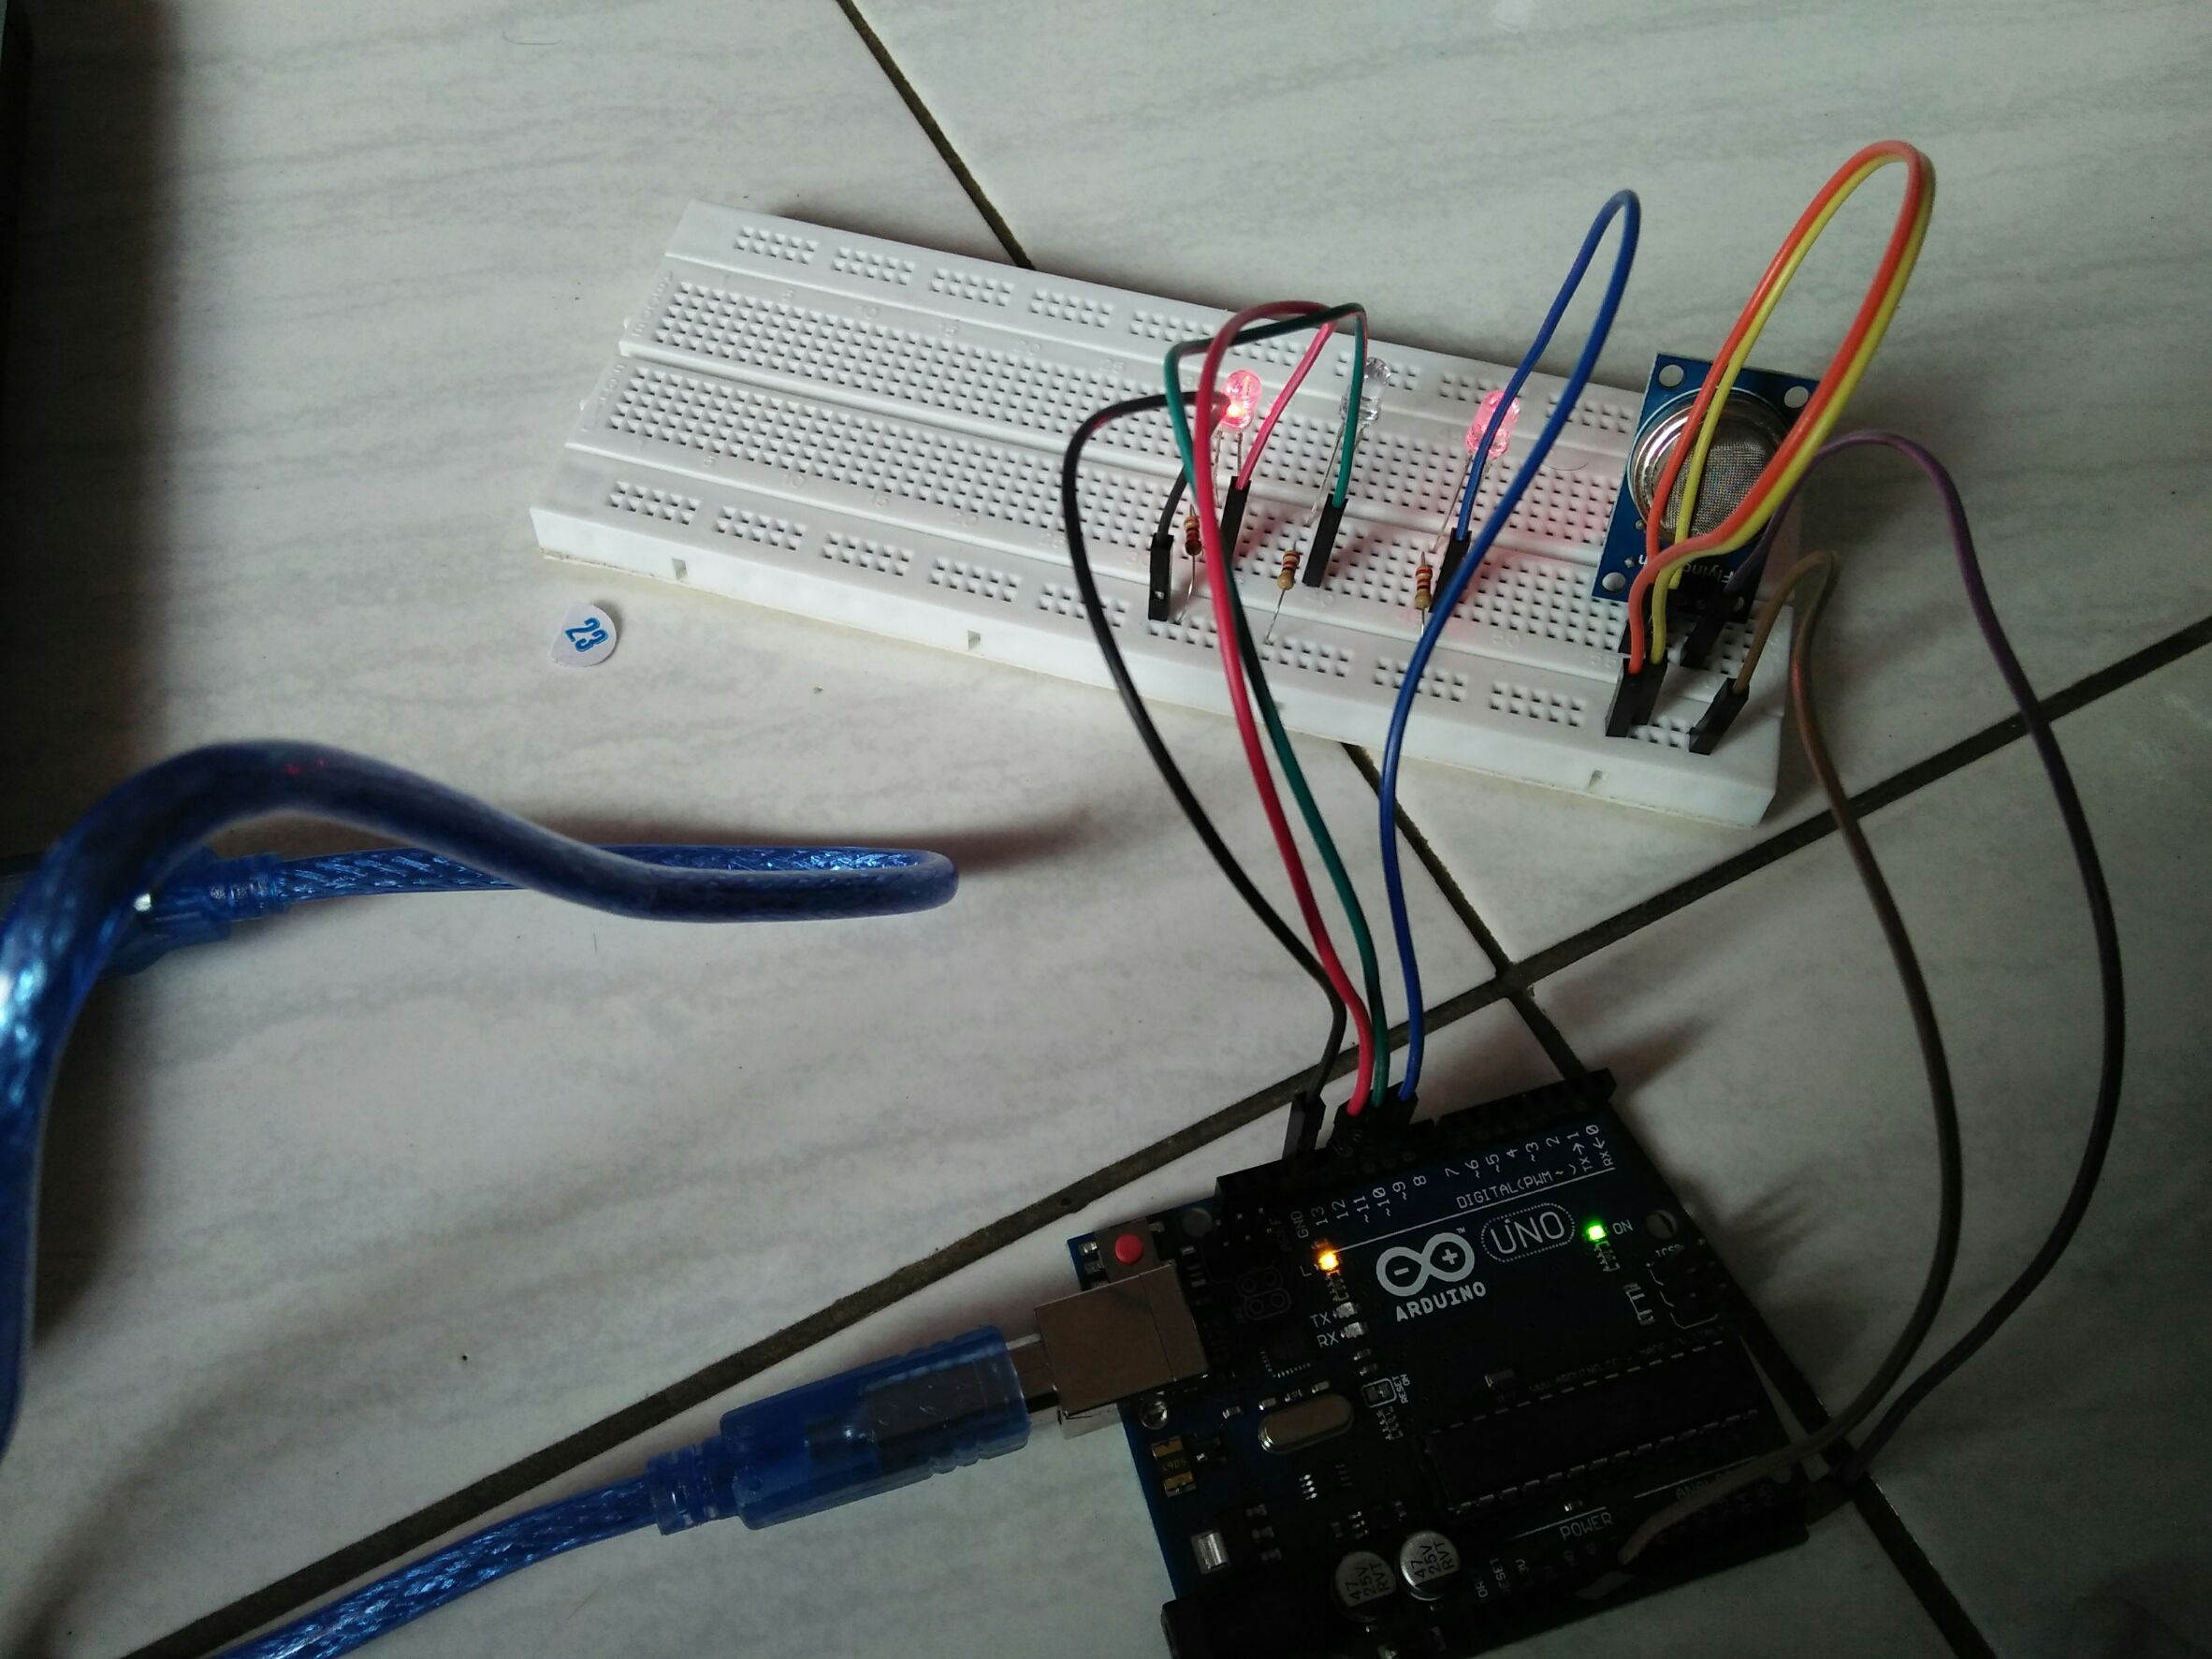
\includegraphics[width=1\textwidth]{figures/terditeksi.jpg}}
	\caption{dua lampu menyala tanda sensor menditeksi gas.}
	\label{sensor:terditeksi}
	\end{figure}
\begin{figure}[ht]
	\centerline{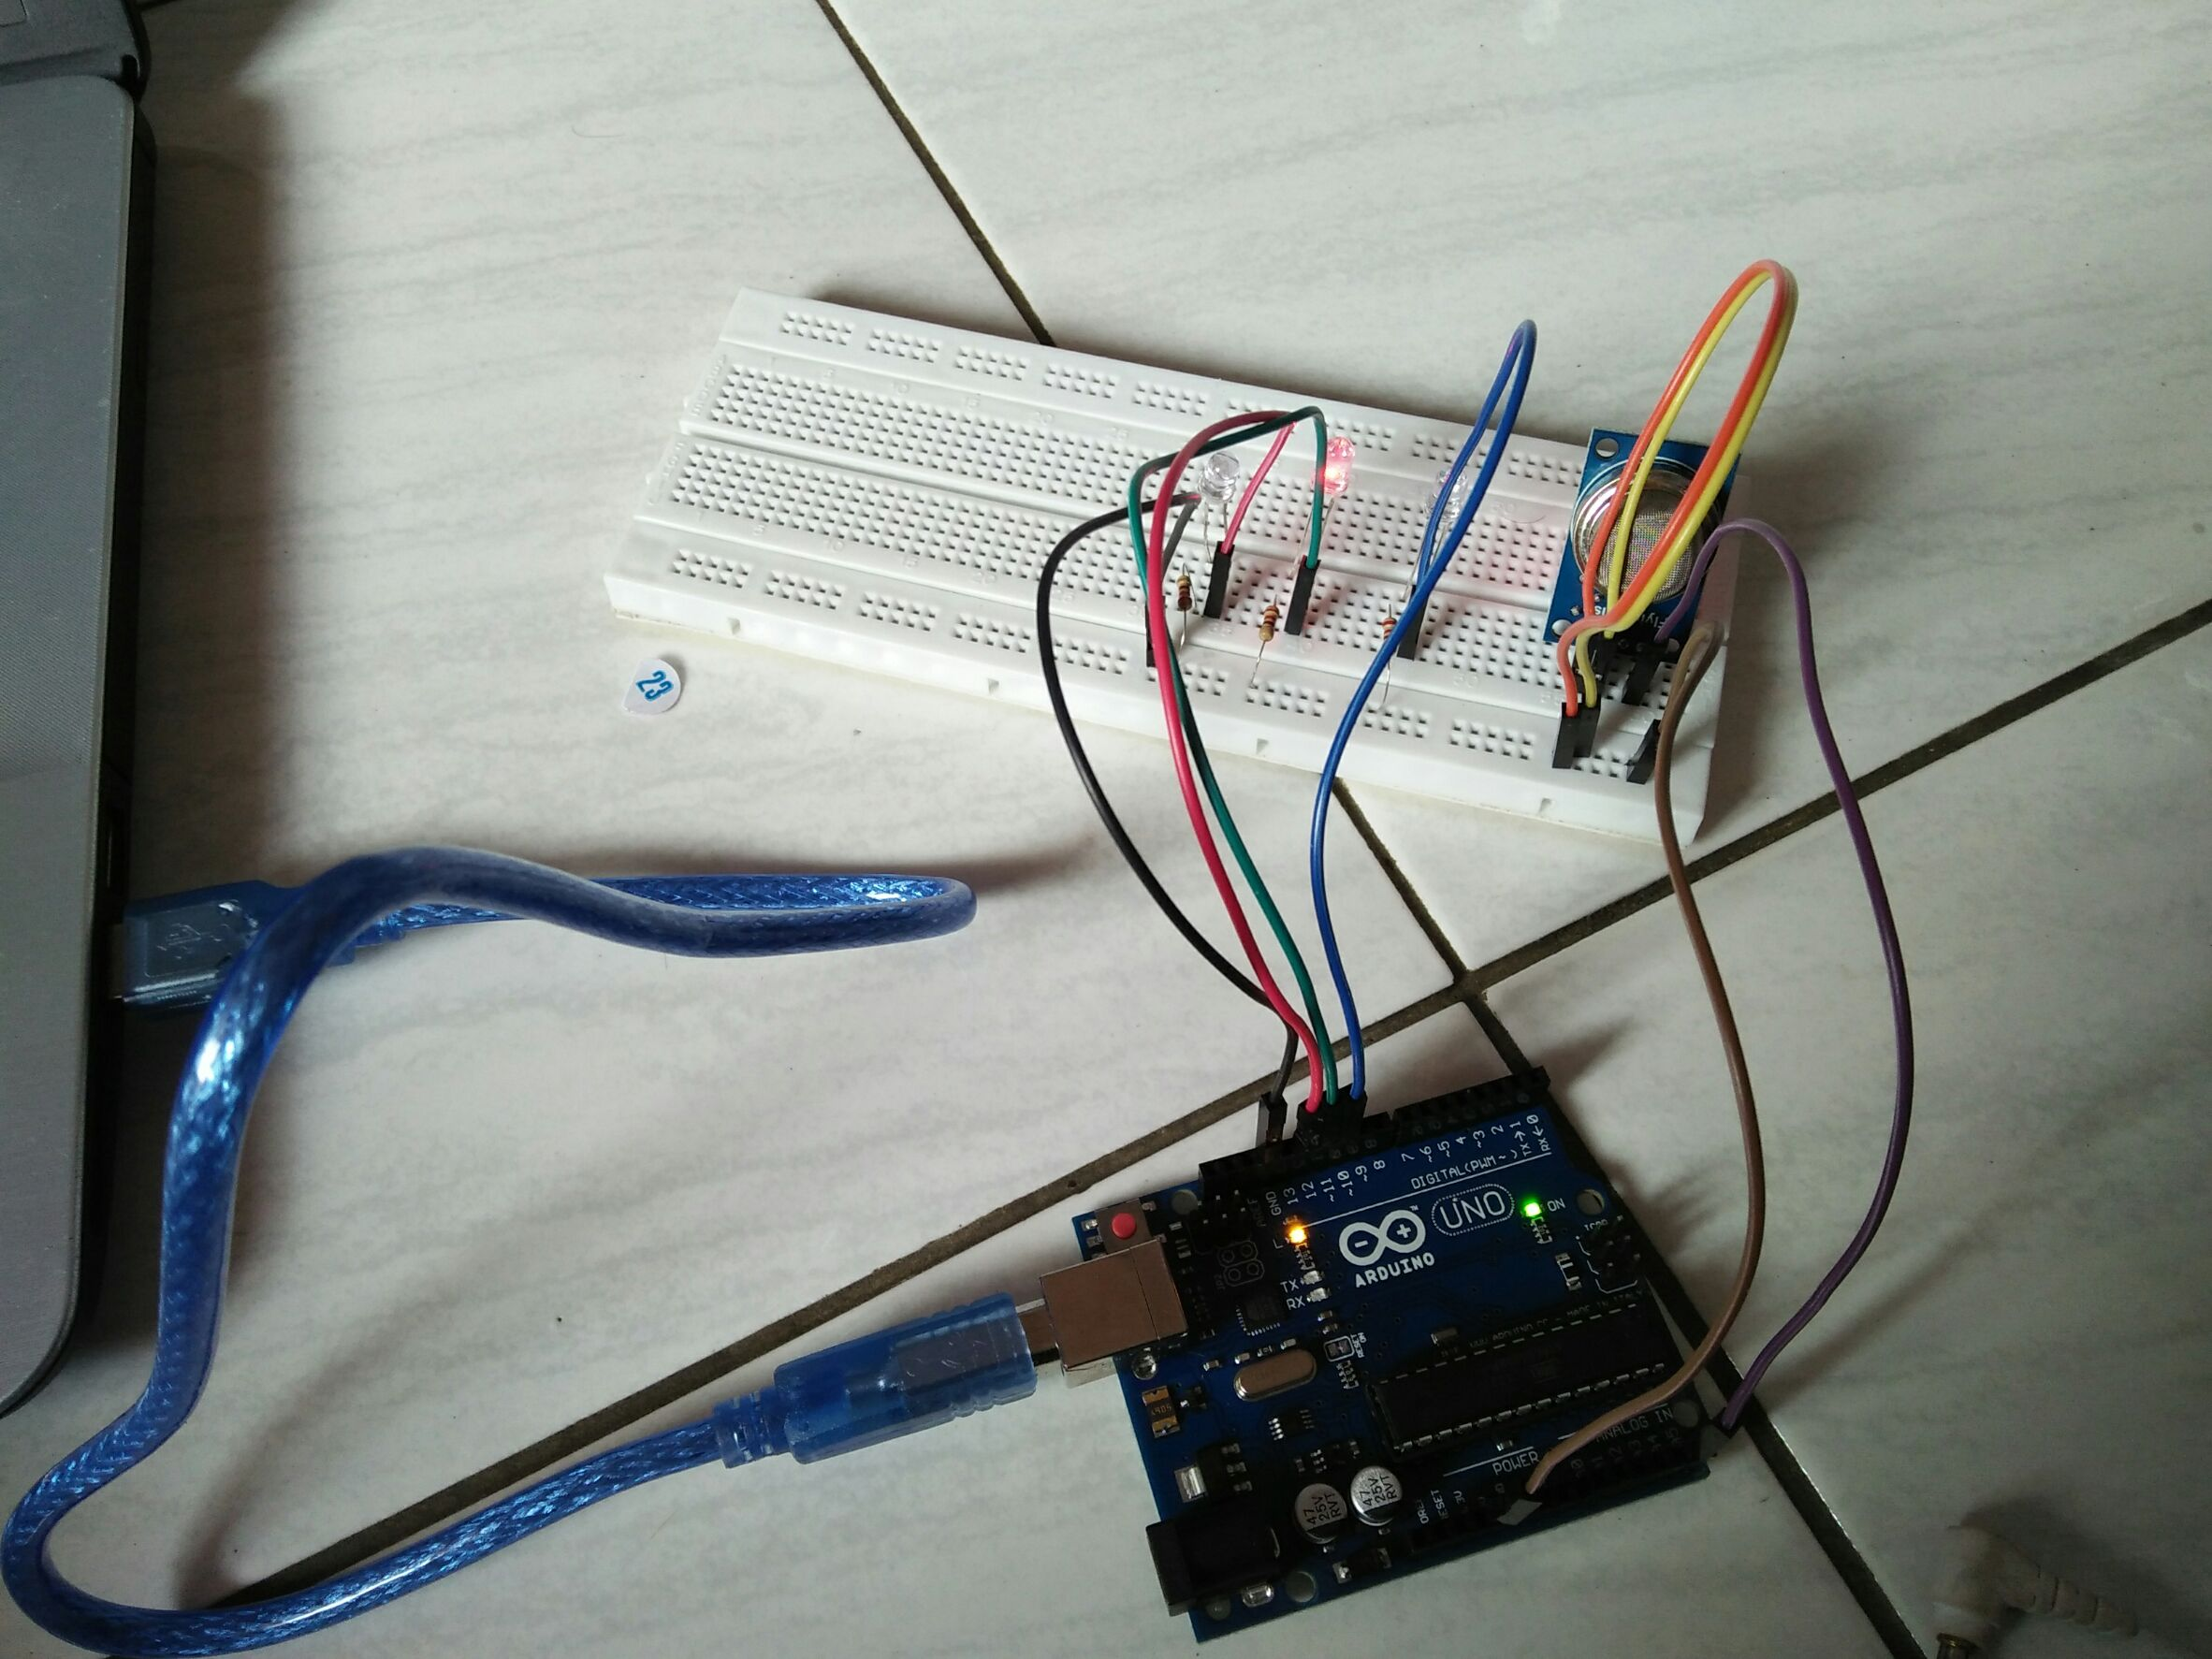
\includegraphics[width=1\textwidth]{figures/tidakterditeksi.jpg}}
	\caption{satu lampu menyala tanda sensor tidak menditeksi gas.}
	\label{sensor:tidakterditeksi}
	\end{figure}
	
Setelah Codingan Berhasil di jalankan maka akan munjul Serial Monitor seperti gambar  \ref{Sensor:SerialMonitor}
\begin{figure}[ht]
	\centerline{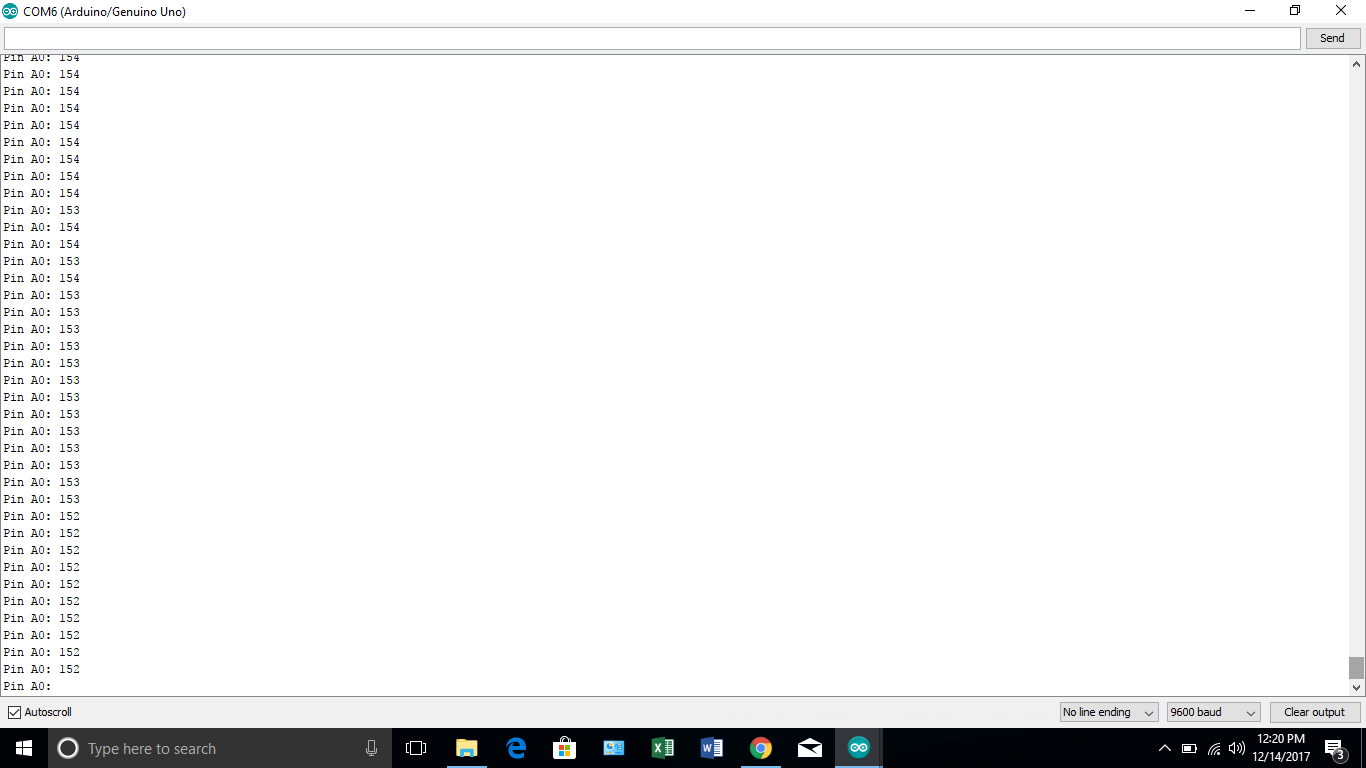
\includegraphics[width=1\textwidth]{figures/SerialMonitor.png}}
	\caption{Serial Monitor Pada Sensor Gas}
	\label{Sensor:SerialMonitor}
	\end{figure}